\subsection*{Venneliste}
Venneliste inddeles i en boundaryklasse og dertilhørende controlklasse, som det fremgår af \autoref{fig:MVCVenneliste}. 

\begin{figure} [H]
\centering
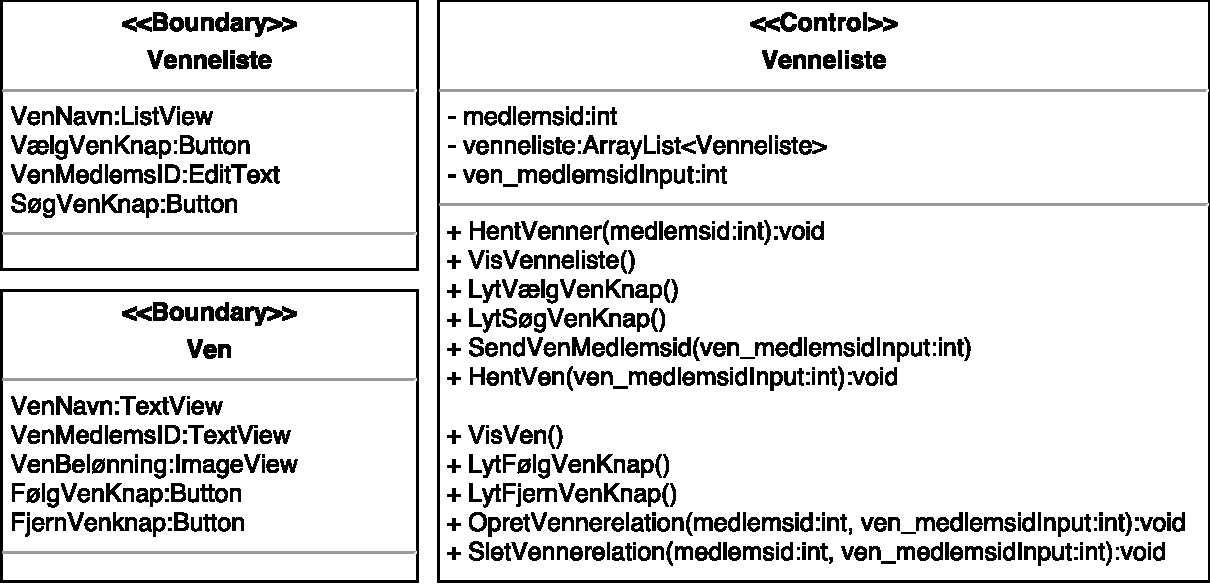
\includegraphics[width=0.8\textwidth]{figures/MVC/MVCVenneliste}
\caption{Designklasser for venneliste.}
\label{fig:MVCVenneliste}
\end{figure}

\noindent
I grænsefladen \textit{Venneliste} findes tekstfelter med fornavn og efternavn på de brugere, der følges. Derudover er der i grænsefladen et tekstfelt, hvori brugeren kan angive medlemsID på andre brugere, der ønskes af følge. Dertil er der to knapper, Søg og Vælg, af typen Button, som controlleren, \textit{Venneliste}, reagerer på. Denne controller har metoderne Hent, Vis og Lyt.

Når en af de to knapper i grænsefladen \textit{Venneliste} trykkes på, vises grænsefladen \textit{Ven}, som indikerer, at en bruger er valgt. Boundaryklassen \textit{Ven} har en tilhørende controlklasse, \textit{Ven}, og disse kan ses af \autoref{fig:MVCVen}.

\begin{figure} [H]
\centering
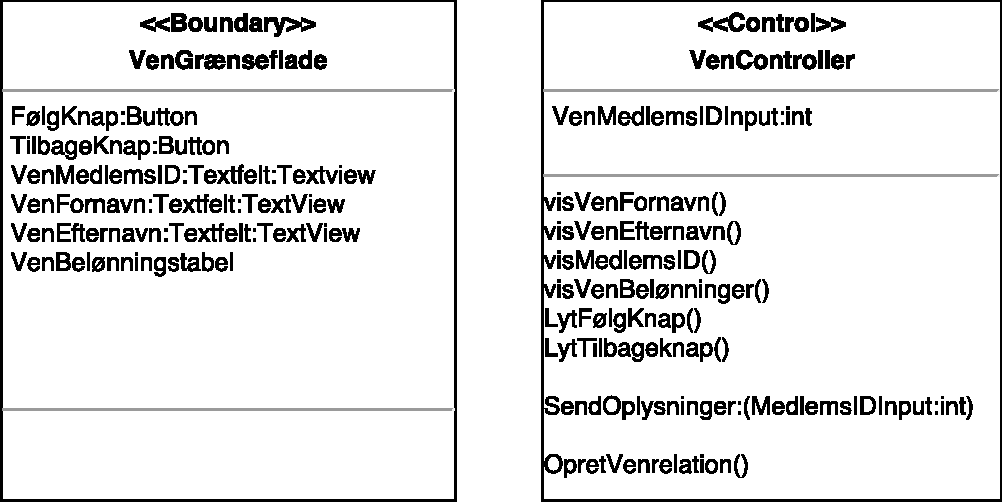
\includegraphics[width=0.8\textwidth]{figures/MVC/MVCVen}
\caption{Designklasser for ven.}
\label{fig:MVCVen}
\end{figure}

\noindent
Boundaryklassen \textit{Ven} indeholder tekstfelter af typen TextView, der viser den valgte brugers medlemsID, fornavn og efternavn. Herudover vises en tabel med den valgte brugers belønninger. Dertil kan der vises knapper af typen Button. Controlklassen \textit{Ven} får input i form af medlemsID, og kan anvende metoderne Vis, Lyt, Hent, Valider og Opret.

Ud fra de nævnte designklasser er udarbejdet et sekvensdiagram, der fremgår af \autoref{fig:SEKVenneliste}.

\begin{figure} [H]
\centering
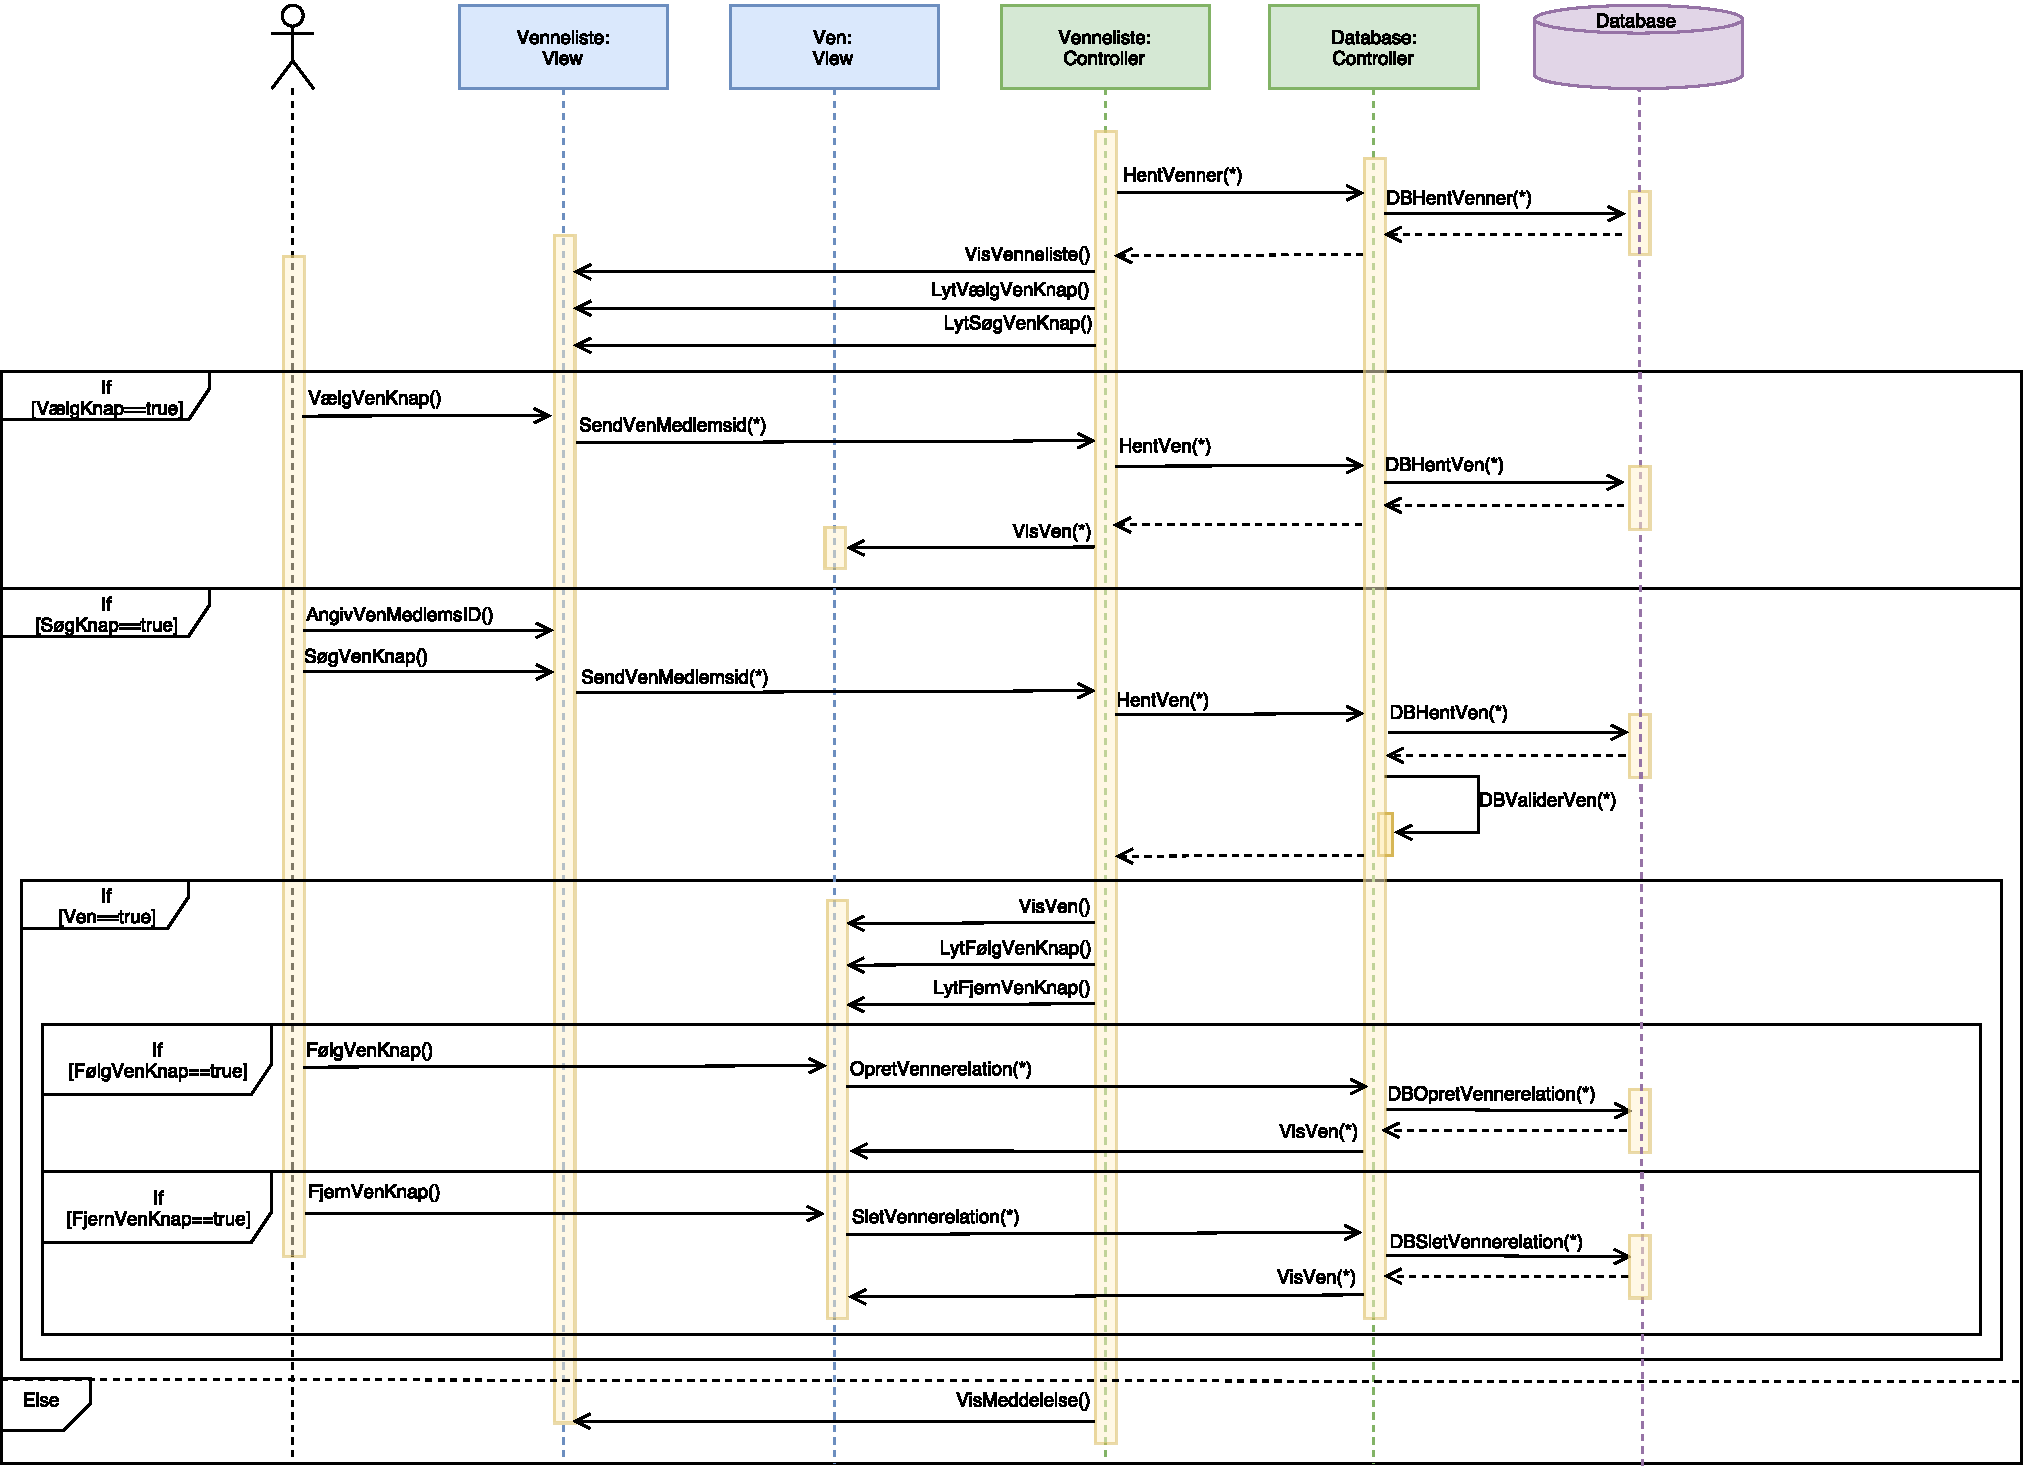
\includegraphics[width=1\textwidth]{figures/Sek/SEKVenneliste}
\caption{Sekvensdiagram for venneliste.}
\label{fig:SEKVenneliste}
\end{figure}

\noindent
Controlleren \textit{Venneliste} henter brugerens venneliste fra modellen \textit{Venneliste}, der beskrives yderligere i \autoref{sec:entity}. Herefter vises vennelisten i grænsefladen \textit{Venneliste}, hvor brugeren har mulighed for at trykke på VælgKnap for at se oplysninger om en enkelt bruger, eller søge på en ny bruger ved at angive dennes medlemsID og trykke på SøgKnap. Controlleren \textit{Ven} lytter på, om brugeren trykker på en af de nævnte knapper.
Trykker brugeren på VælgKnap, viser controlleren \textit{Ven} oplysninger om den valgte bruger i grænsefladen \textit{Ven}.
Trykker brugeren på SøgKnap, henter \textit{VenController} oplysninger om det indtastede medlemsID i \textit{Database}, hvorefter medlemsID'et valideres. Hvis medlemsID'et findes i databasen, viser controlleren oplysninger om den søgte bruger i grænsefladen \textit{Ven}. Brugeren har herefter mulighed for at trykke på FølgKnap, og hvis dette er tilfældet, opretter \textit{VenController} en vennerelation i \textit{Database}. Hvis medlemsID'et ikke findes i databasen, viser controlleren en fejlmeddelelse i grænsefladen \text{Fejlmeddelelse}, og brugeren kan trykke på OKKnap, hvorefter \textit{VenControlleren} viser grænsefladen \textit{Venneliste}. 

SKAL OK-KNAPPEN STADIG VÆRE I DENNE GRÆNSEFLADE?









%Venneliste inddeles i en grænseflade og dertilhørende controller, som det fremgår af \autoref{fig:MVCVenneliste}. 

%\begin{figure} [H]
%\centering
%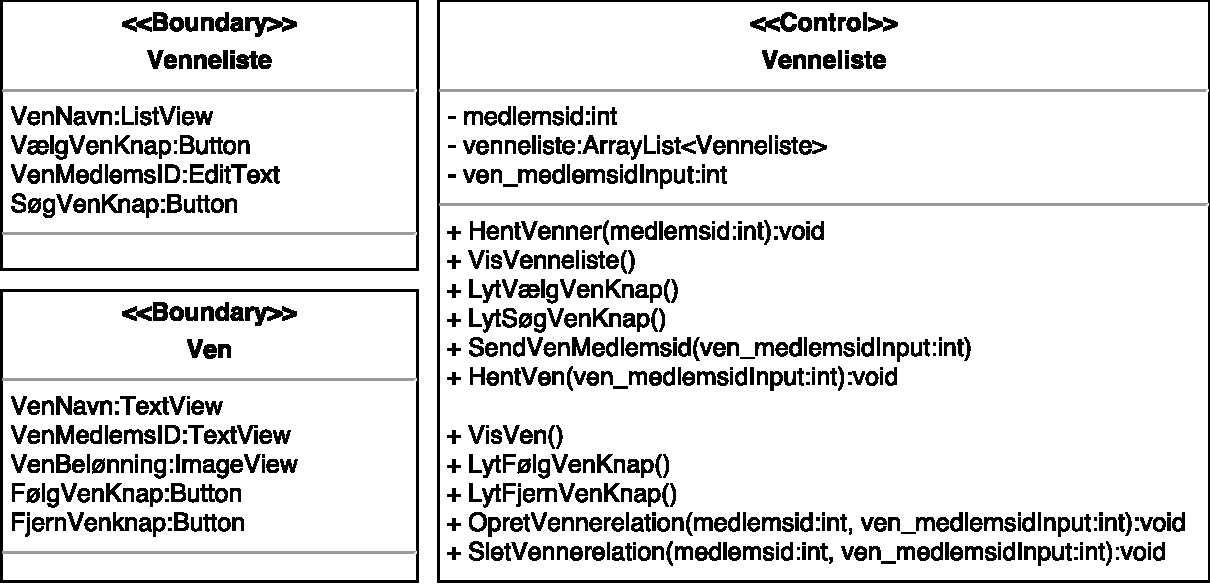
\includegraphics[width=0.8\textwidth]{figures/MVC/MVCVenneliste}
%\caption{Designklasser for venneliste.}
%\label{fig:MVCVenneliste}
%\end{figure}

%\noindent
%\textit{VennelisteGrænsefladen} indeholder tekstfelter for fornavn og efternavn på de brugere de følger. Derudover er der opstillet tekstfelt for medlemsID, hvor brugeren kan angive medlemsID'et på en bruger de ønsker at følge. Dertil er der opstillet en tilhørende søge knap, af typen button, der ved tryk indikere at brugeren har angivet medlemsID på brugeren den ønsker at følge. Derudover har brugeren mulighed for at vælge en bruger eller gå tilbage via en vælg eller tilbage  knap, der også er af typen button. 


%Der er til \textit{VennelisteGrænsefladen} opstillet en \textit{VennelisteController}, der har til formål at vise en oversigt over vennelisten når grænsefladen for vennelisten tilgås. Brugeren har via vælg knappen mulighed for at tilgå en bruger den følger
%Controlleren lytter på om brugeren trykker på vælg knappen eller søg knappen. Vælg knappen giver brugeren mulighed for at tilgå enkelt bruger ud fra vennelisten. Trykker brugeren på søg knappen kontrollere controlleren om det angivne medlemsID findes i databasen, herefter kan brugeren trykke på vælg. Trykkes der på en af vælg knapperne, enten i vennelisten eller efter søgning på medlemsID vises \textit{VenGrænsefladen}, som fremgår af \autoref{MVCVen}. Controlleren lytter på tilbage knappen, hvis denne trykkes på vises forrige grænseflade. 


%\subsubsection*{Ven}
%Ven inddeles i en grænseflade og tilhørende controller, som det fremgår af \autoref{fig:MVCVen}.

%\begin{figure} [H]
%\centering
%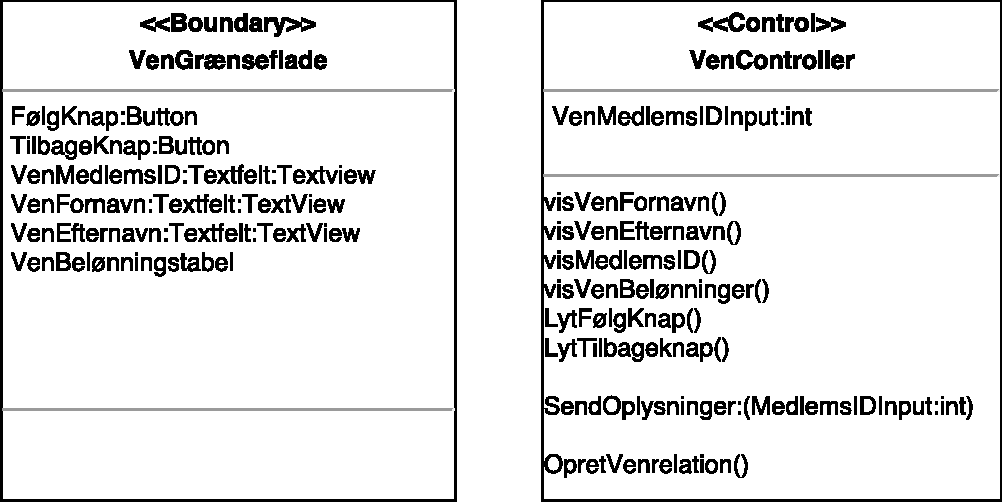
\includegraphics[width=0.8\textwidth]{figures/MVC/MVCVen}
%\caption{Designklasser for ven.}
%\label{fig:MVCVen}
%\end{figure}

%\noindent
%I \textit{VenGrænseflade} vises tekstfelter for valgt bruger, herunder MedlemsID, fornavn og efternavn. Dertil er der opstillet en følg knap og en tilbage knap af typen button. Følg knap er kun tilgængelig, hvis brugeren ikke følger den valgte ven. Derudover vises en tabel med den valgte brugers belønninger.


%Til \textit{VenGrænsefladen} er der opstillet en \textit{VenController}, som har til formål vise brugeroplysninger, herunder MedlemsID, fornavn og efternavn samt belønningstabel for den valgte bruger. Controlleren lytter på om brugeren trykker på følg knappen, hvis brugeren ikke allerede følger eller trykker på tilbage knappen. Trykkes der på følg knappen sendes MedlemsID'et på den bruger der ønskes at følges til databasen, hvorefter vennerelation gemmes i denne. Vælger brugeren at trykke på tilbage knappen vises den forrige grænseflade.   